\chapter{MOSFET Operation}
MOSFET stands for Metal Oxide Semiconductor Field Effect Transistor. 
\begin{figure}[H]
\centering
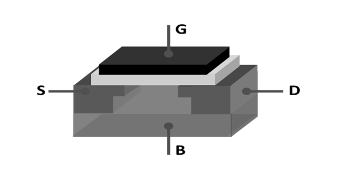
\includegraphics[scale=0.5]{./fig21} % e.g. insert ./image for image.png in the working directory, adjust scale as necessary
\caption{Simple diagram of a MOSFET}
\label{3.21} % insert suitable label, this is used to refer to a fig from within the text as shown above
\end{figure}
 
\noindent A MOSFET comprises of an Oxide layer sandwiched between a metal contact (or Polysilicon) and a semiconductor (Bulk Si). It controls current flow using an electric field applied via the Gate terminal and is therefore called a Field Effect Transistor. Carriers flow from the Source to Drain which are heavily doped semiconductors diffused into the bulk.

\section{Working of a MOSFET and IV Characteristics}
Let us consider a MOSFET with p-type bulk Si and heavily doper n-type Si at the source and drain. Initially, let gate and substrate voltage be 0 and VDD be applied to drain. As source-substrate and drain-substrate junctions are reverse biased, no current flows. We refer to this region as sub-threshold region

\begin{figure}[H]
\centering
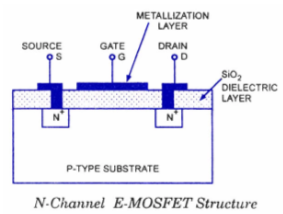
\includegraphics[scale=0.5]{./fig22} % e.g. insert ./image for image.png in the working directory, adjust scale as necessary
\caption{An N-channel enhancement mode MOSFET}
\label{3.22} % insert suitable label, this is used to refer to a fig from within the text as shown above
\end{figure}
 
 
\noindent Upon application of a gate voltage, the positive voltage attracts electrons and repels holes in the substrate. Repelled holes and incoming electrons recombine to form Si atoms. However, after a certain threshold is crossed, the accumulation of electrons overwhelms recombination. At and beyond this value of threshold gate voltage, electrons form a majority below the gate oxide and form a thin channel.

\begin{figure}[H]
\centering
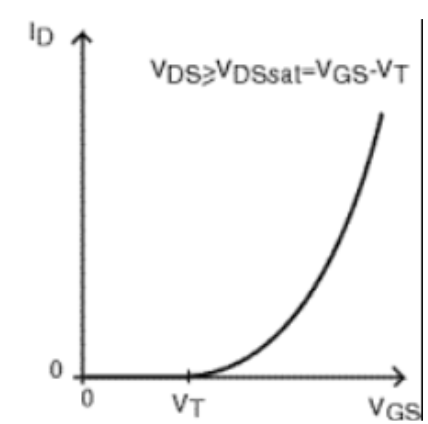
\includegraphics[scale=0.5]{./fig23} % e.g. insert ./image for image.png in the working directory, adjust scale as necessary
\caption{Drain current plotted as a function of gate voltage}
\label{3.23} % insert suitable label, this is used to refer to a fig from within the text as shown above
\end{figure}
 

\noindent As this channel is composed of electrons, it is known as an n-type channel and hence an n-type MOSFET. Also, the gate voltage enhances the concentration of n-type carriers and it is therefore an enhancement-mode MOSFET. Beyond the threshold voltage, there is a very low-resistance path for the drain current that is produced by the voltage at drain. The channel acts as a linear resistor and therefore drain current increases linearly with drain voltage. This is known as non-saturation region. 

\begin{figure}[H]
\centering
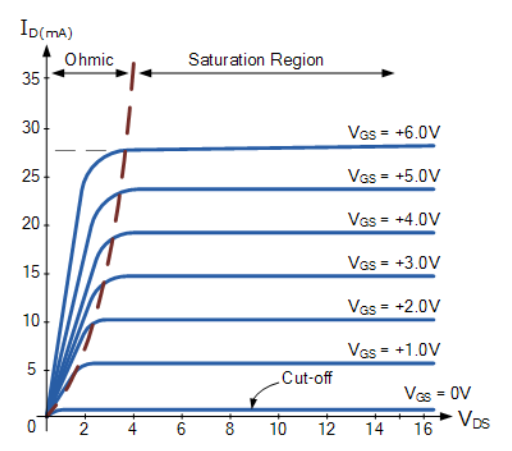
\includegraphics[scale=0.5]{./fig24} % e.g. insert ./image for image.png in the working directory, adjust scale as necessary
\caption{Drain current plotted against drain voltage}
\label{3.24} % insert suitable label, this is used to refer to a fig from within the text as shown above
\end{figure}

\noindent However, with an increase in drain voltage, the potential drop between the source and drain decreases. This reduction in potential drop across the channel lowers its width. Also, increase in drain voltage attracts n-type carriers away from the channel producing a pinch off and increasing the width of depletion region. A wider depletion region imposes greater resistance and thus drain current remains constant in spite of increasing voltage. This is known as saturation region.

\section{CV Characteristics}
\begin{figure}[H]
\centering
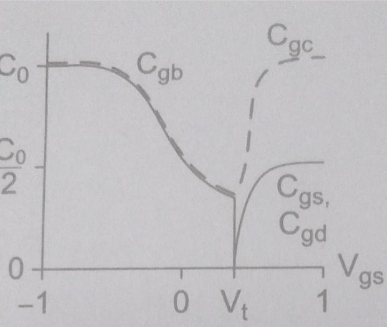
\includegraphics[scale=0.5]{./fig25} % e.g. insert ./image for image.png in the working directory, adjust scale as necessary
\caption{Capacitance plotted against gate voltage}
\label{3.25} % insert suitable label, this is used to refer to a fig from within the text as shown above
\end{figure}

Under no gate bias, the capacitance of the MOSFET equals the oxide capacitance formed between metal contact and the substrate. capacitance due to depletion regions is zero as none are formed. As gate bias is increased and channel formation begins, the effective distance between the plates increases reducing the capacitance. Upon formation of channel, for low values of drain voltage, capacitance between gate to source and gate to drain is equal hence C0/2 as they are in series.
